%======================================================================
\chapter{Methodology}
\label{chapter:methodology}
%======================================================================

%Go into detail about the methods used in doing your project/thesis. What are the relevant ideas, the sources of information, the various approaches that might be used? Discuss approaches finally chosen as well as those discarded and finally describe what was accomplished. It is important here to strike a balance between too much detail and not enough. Above all, avoid a repetitious style. This part of the report is usually covered in one or more middle chapters. A good rule-of-thumb is to break a chapter into two or more parts if it is large compared to other chapters.

This chapter will discuss the various methods and algorithms used in this project in order to generate randomized graphs and their data. Each section discusses a certain generation process, as well as its applied use cases. 


\section{Midpoint Displacement}
One of the first algorithms explored was Midpoint Displacement, also known as the Diamond-square Algorithm. As seen in \autoref{figure:midpoint_landscape}, this method is typically used for 2-D mountainous landscape generation.

\hfill

\begin{figure}[hbt]
    \centering
    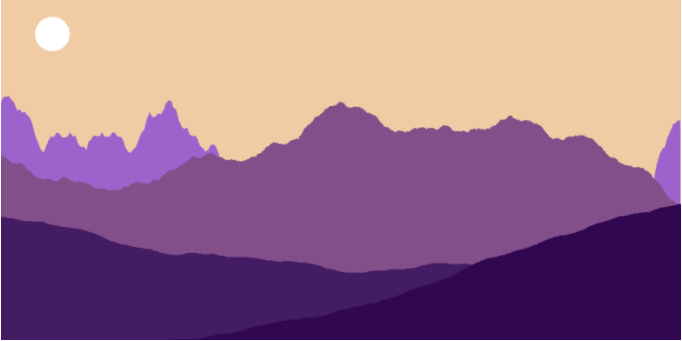
\includegraphics[width=250pt,keepaspectratio]{figures/body/methodology/MD_2D_landscape.PNG}
    \caption{Example Midpoint Displacement Landscape Generation \cite{acin_2016}}
    \label{figure:midpoint_landscape}
\end{figure}

\subsection{Generation}
Midpoint Displacement begins by simply initializing a straight line segment. After computing the segment's midpoint, it then displaces the \(y\) coordinate value by a ``bounded random value" \cite{acin_2016}. This process is then iterated over as many times as desired, reducing the bounded displacement value each time. This has the effect of creating twice as many segments in every iteration. Successive steps of the Midpoint Displacement algorithm result in segments similar to the image shown in \autoref{figure:midpoint_algorithm}.

\hfill

\begin{figure}[hbt]
    \centering
    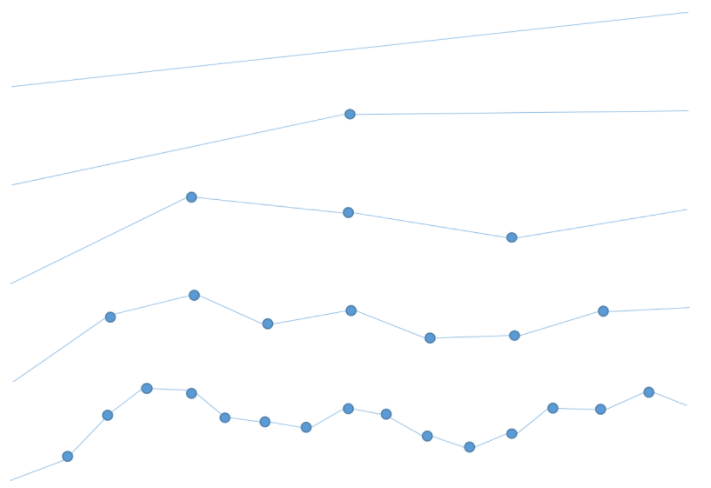
\includegraphics[width=250pt,keepaspectratio]{figures/body/methodology/MD_line_segments.PNG}
    \caption{Iterations of Midpoint Displacement Algorithm \cite{acin_2016}}
    \label{figure:midpoint_algorithm}
\end{figure}

\subsection{Use Cases}
Midpoint Displacement was applied for area charts, line graphs, and error bar charts. These were chosen because their correlation of data tends to be visually similar in terms of mountainous peaks and ranges.

\hfill

To execute this, each graph was given randomly generated parameters such as the number of layers, number of iterations, vertical displacement and roughness (\autoref{section:random_number_generation}). These parameters were then fed into a Midpoint Displacement algorithm that randomly generated \(X\) and \(y\) points for each line, or layer. 

\hfill

A key difference between these types of graphs is that the area charts required the \(y\) coordinates to be ``stacked" on top of each other, such that no lines crossed over each other. This stacking effect is displayed in section \autoref{figure:area_plot}. Moreover, line graphs required less ``jagged peaks" in their display, and so the range of roughness was decreased, as well as the number of iterations. As seen in \autoref{figure:line_graph} and \autoref{figure:error_bar}, this resulted in smoother-looking correlations, with less points per line. Error bar graphs were formatted in a similar manner to line graphs, but with randomly-generated lengths for the error bars at each point. It is also worth nothing that line graphs and error bar graphs had a 50\% chance of implementing Random Number Generation instead of just Midpoint Displacement, which will be further discussed in \autoref{section:random_number_generation}. 

\hfill

\begin{figure}
    \centering
    \begin{subfigure}[b]{0.32\textwidth}
        \centering
        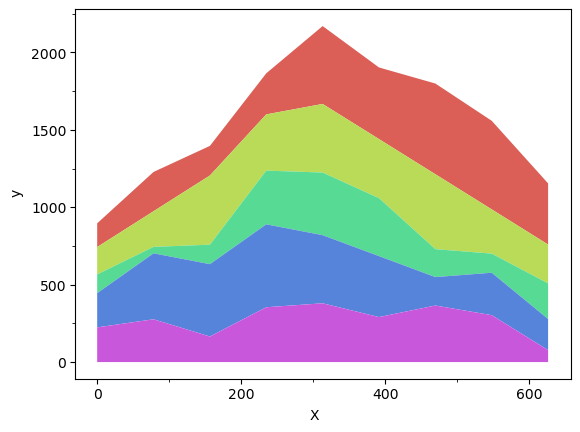
\includegraphics[width=\textwidth]{figures/body/methodology/MD_area.png}
        \caption{Area Plot}
        \label{figure:area_plot}
    \end{subfigure}
    \hfill
    \begin{subfigure}[b]{0.32\textwidth}
        \centering
        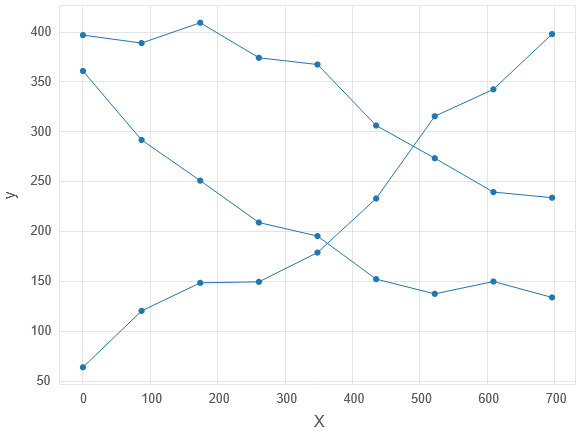
\includegraphics[width=\textwidth]{figures/body/methodology/MD_line.png}
        \caption{Line Graph}
        \label{figure:line_graph}
    \end{subfigure}
    \hfill
    \begin{subfigure}[b]{0.32\textwidth}
        \centering
        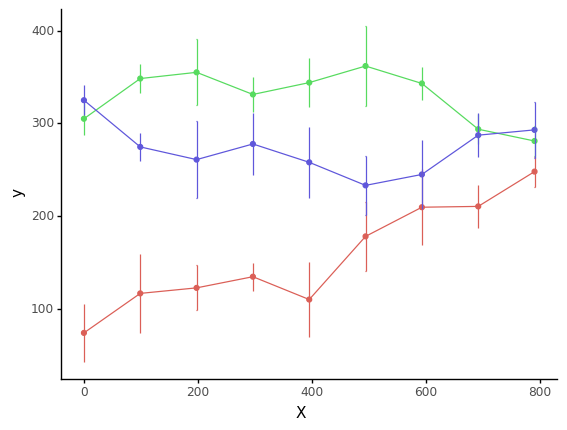
\includegraphics[width=\textwidth]{figures/body/methodology/MD_errorbar.png}
        \caption{Error Bar}
        \label{figure:error_bar}
    \end{subfigure}
    \caption{Midpoint Displacement Chart Generation}
    \label{figure:midpoint_generation}
\end{figure}

\section{Regression}
Both Linear and Logarithmic Regression were implemented in order to generate a correlation effect in non-categorical graphs such as scatter plots and bubble plots.

\subsection{Generation}
Linear Regression's data points visually form the shape of a line, which follows the algorithm \(y = mx +b\), where \(m\) is the given slope and \(b\) is some given intercept. The generation of positive Linear Regression was implemented through the use of \href{https://scikit-learn.org/stable/}{scikit-learn}'s \path{make_regression()} method, which returns a number of \(X\) and \(y\) values. Its input parameters of the number of samples, number of features, noise level, and tail strength were all randomly generated within a set range (\autoref{section:random_number_generation}). Negative Linear Regression follows the same process, but all \(y\) values are negated.

\hfill

Although the \(X\) values are still created with scikit-learn's \path{make_regression()} method, Logarithmic Regression requires that \(x>0\), and so all invalid data is filtered out and replaced. Furthermore, unlike Linear Regression, the creation of each \(y\) value is mapped to the logarithm of its matching \(X\) value. This results in an equation similar to \(y = log(x)\). In this project, each calculation has a random logarithmic base, which ranges between two values specified in the generation's parameters (\autoref{section:random_number_generation}). If the Logarithmic Regression results in a negative correlation, these \(y\) values will then be negated.

\subsection{Use Cases}

Linear Regression was utilized for generating both scatter plots and bubble plots. Various noise is randomly applied to each generation, resulting in the graphs ranging from seemingly straight lines to no visible correlation. This variation in noise is displayed through the scatter plots shown in \autoref{figure:scatterplot_noise_regression}.

\hfill

% Noise in Positive Linear Regression - Scatter Plot
\begin{figure}
    \centering
    \begin{subfigure}[b]{0.19\textwidth}    
        \centering
        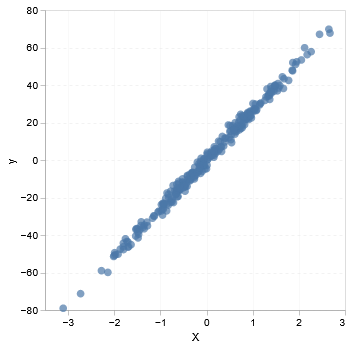
\includegraphics[width=\textwidth]{figures/body/methodology/linear_scatter1.png}
        \label{figure: scatter1}
        \caption{\(x = 2.09\)}
    \end{subfigure}
    \hfill
    \begin{subfigure}[b]{0.19\textwidth}
        \centering
        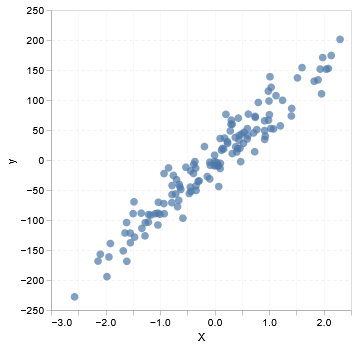
\includegraphics[width=\textwidth]{figures/body/methodology/linear_scatter2.png}
        \label{figure: scatter2}
        \caption{\(x = 25.18\)}
    \end{subfigure}
    \hfill
    \begin{subfigure}[b]{0.19\textwidth}
        \centering
        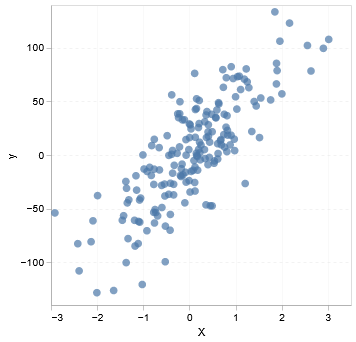
\includegraphics[width=\textwidth]{figures/body/methodology/linear_scatter3.png}
        \label{figure: scatter3}
        \caption{\(x = 29.72\)}
    \end{subfigure}
    \hfill
    \begin{subfigure}[b]{0.19\textwidth}
        \centering
        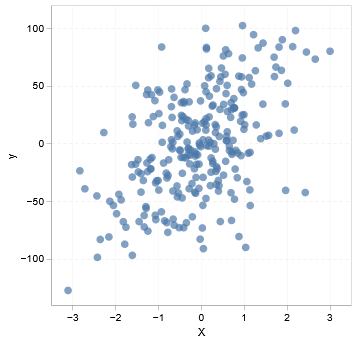
\includegraphics[width=\textwidth]{figures/body/methodology/linear_scatter4.png}
        \label{figure: scatter4}
        \caption{\(x = 40.17\)}
    \end{subfigure}
    \hfill
    \begin{subfigure}[b]{0.19\textwidth}
        \centering
        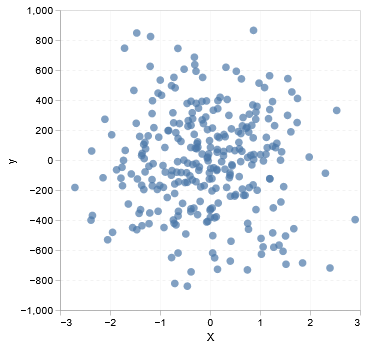
\includegraphics[width=\textwidth]{figures/body/methodology/linear_scatter5.png}
        \label{figure: scatter5}
        \caption{\(x = 355.77\)}
    \end{subfigure}
    \caption{Noise in Positive Linear Regression - Scatter Plot}
    \label{figure:scatterplot_noise_regression}
\end{figure}

In addition to Linear Regression, bubble plots have a 50\% chance to follow Logarithmic Regression when being generated. This difference in pattern can be clearly seen in \autoref{figure:bubbleplot_regression}, which displays the two types of regressions as bubble plots. Other than the inclusion of logarithms, an important distinction between bubble and scatter plots is that bubble plots also required a random generation of bubble size, which is discussed later in \autoref{section:random_number_generation}.

\hfill

\begin{figure}
    \centering
     \begin{subfigure}[b]{0.21\textwidth}
         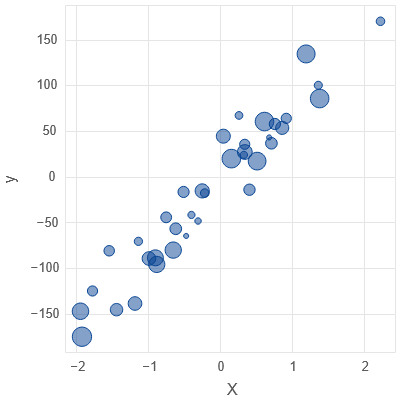
\includegraphics[width=\textwidth]{figures/body/methodology/linear_pos_bubble.png}
         \caption{Positive Linear}
         \label{figure: pos_lin}
     \end{subfigure}
     \hfill
     \begin{subfigure}[b]{0.21\textwidth}
         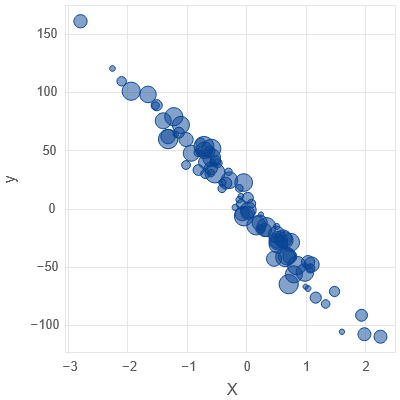
\includegraphics[width=\textwidth]{figures/body/methodology/linear_neg_bubble.png}
         \caption{Negative Linear}
         \label{figure: neg_lin}
     \end{subfigure}
     \hfill
     \begin{subfigure}[b]{0.21\textwidth}
         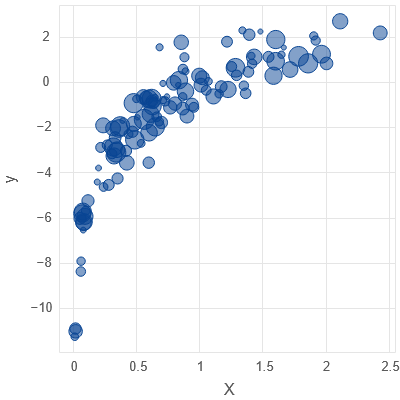
\includegraphics[width=\textwidth]{figures/body/methodology/log_pos_bubble.png}
         \caption{Positive Log}
         \label{figure: pos_log}
     \end{subfigure}
     \hfill
     \begin{subfigure}[b]{0.21\textwidth}
         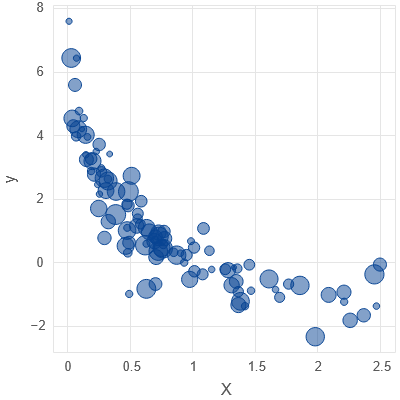
\includegraphics[width=\textwidth]{figures/body/methodology/log_neg_bubble.png}
         \caption{Negative Log}
         \label{figure: neg_log}
     \end{subfigure}
        \caption{Linear and Logarithmic Regression - Bubble Plot}
        \label{figure:bubbleplot_regression}
\end{figure}

\section{Distribution Sampling}
%do we need a tag here

The process of sampling values from a provided statistical distribution is known as distribution sampling. The distributions discussed below are Continuous Probability Distributions, most of which are implemented using Python's \href{https://numpy.org/}{NumPy} library. These distributions are repeatedly sampled to create a set of datapoints based on an underlying distribution. In this context, the term ``Continuous" refers to the ``probabilities of the possible values of a continuous random variable", where each random variable has a range of possible values \cite{minitab_express}. Furthermore, each type of Continuous Probability Distribution follows a Probability Density Function, which is used to calculate the probabilities of continuous random variables. 

\subsection{Generation}
As many types of graphs utilize Continuous Probability Distributions for data generation, this section will discuss a wide variety of these distribution types. Specifically Gaussian Distribution, Log-normal Distribution, Gamma Distribution, Weibull Distribution, Uniform Distribution, and Multivariate Gaussian Distribution will be covered.

\subsubsection{Gaussian Distribution}
\label{subsubsection:normal_distribution}
Gaussian Distribution, also termed Normal Distribution, is a symmetrical distribution. The correlation forms a shape that is often described as a ``bell curve", which is a result of its centralized mean. With \(\mu\) as the mean and \(\sigma\) as standard deviation, Gaussian Distribution follows the Probability Density Function shown below:

\begin{displaymath}
f(x) = \frac{1}{\sigma\sqrt{2\pi}}e^{\frac{-1}{2}(\frac{x-\mu}{\sigma})^2}
\end{displaymath}

\hfill

The data generation for Gaussian Distribution was created through NumPy's \path{random.normal()} method, which takes input parameters for the mean and standard deviation of the distribution. These required values were randomly generated within a predetermined range for each graph (\autoref{section:random_number_generation}).


\subsubsection{Log-normal Distribution}
Visually similar to Gaussian Distribution (\autoref{subsubsection:normal_distribution}), Log-normal Distribution is identifiable by having a right-skewed bell curve, which results in a non-symmetrical shape. As the name suggests, a Log-normal Distribution is ``a continuous distribution of random variable \(y\) whose natural logarithm is normally distributed" \cite{KISSELL2017103}. With \(\mu\) as the mean and \(\sigma\) as standard deviation, Log-normal Distribution satisfies the following Probability Density Function: 

\begin{displaymath}
f(x) = \frac{1}{\sigma\sqrt{2\pi}}e^{\frac{-1}{2}(\frac{lnx-\mu}{\sigma})^2}
\end{displaymath}

\hfill

Rather than using NumPy's \path{random.normal()} function, graphs following a Log-normal Distribution utilize \path{random.lognormal()} instead. The input parameters remain the same as the ones used for Gaussian Distribution (\autoref{subsubsection:normal_distribution}).

\subsubsection{Gamma Distribution}
Gamma Distribution is a maximum entropy probability distribution that is skewed rightwards. It fits the Probability Density Function displayed below, with \(k\) as the shape parameter, \(\theta\) as the scale parameter, and \(\Gamma\) as the gamma function, which can be defined as an ``extension of the factorial function to real (and complex) numbers" \cite{glen_2014}:

\begin{displaymath}
f(x) = \frac{1}{\Gamma(k)\theta^k}x^{k-1}e^{-\frac{x}{\theta}}
\end{displaymath}

\hfill

Data for Gamma Distribution was generated through the use of NumPy's \path{random.gamma()} method, which received randomized values within a specified range for its required input parameters of shape and scale (\autoref{section:random_number_generation}). 


\subsubsection{Uniform Distribution}
\label{subsubsection:uniform_distribution}
A Uniform Distribution is one in which every result, within a certain maximum and minimum bounds, is equally likely. This results in a fairly constant-looking correlation, with no noticeable peaks or skews. With \(a\) as the minimum and \(b\) as the maximum such that \(a\le x\le b\), Uniform Distribution fits the Probability Density Function displayed below:

\begin{displaymath}
f(x) = \frac{1}{b-a}
\end{displaymath}

\hfill

Generation for Uniform Distribution was performed with NumPy's \path{random.uniform()} method. The required input parameters of the minimum and maximum were randomly generated within a specified range (\autoref{section:random_number_generation}).

\subsubsection{Weibull Distribution}
Related to exponential functions, Weibull Distribution takes \(k\) as the shape parameter and \(\lambda\) as the scale parameter in order to satisfy the following Probability Density Function:

\begin{displaymath}
f(x) = \begin{cases} \frac{k}{\lambda}(\frac{x}{\lambda})^{k-1}e^{-(\frac{x}{\lambda})^k}, & x \ge 0 \\ 0, & x < 0 \end{cases}
\end{displaymath}

\hfill

The data generation process for Weibull Distribution involved using NumPy's \path{random.uniform()} method to initially generate a Uniform Distribution (\autoref{subsubsection:uniform_distribution}). This Uniform Distribution data, represented as \(d\), was then placed into the following equation: 

\begin{displaymath}
data = \lambda(-log(d))^{\frac{1}{k}}
\end{displaymath}

\hfill

As seen, this equation transforms the Uniform Distribution into a Weibull Distribution final data array through the use of NumPy's \path{log()} function, as well as the randomized input of the shape parameter \(k\), and the scale parameter \(\lambda\) (\autoref{section:random_number_generation}).


\subsubsection{Multivariate Gaussian Distribution}
Also named Multivariate Normal Distribution, Multivariate Gaussian Distribution place Gaussian Distributions (\autoref{subsubsection:normal_distribution}) into a multi-dimensional format. This is clearly visualized in \autoref{figure:multivariate_normal}.

\begin{figure}[hbt]
    \centering
    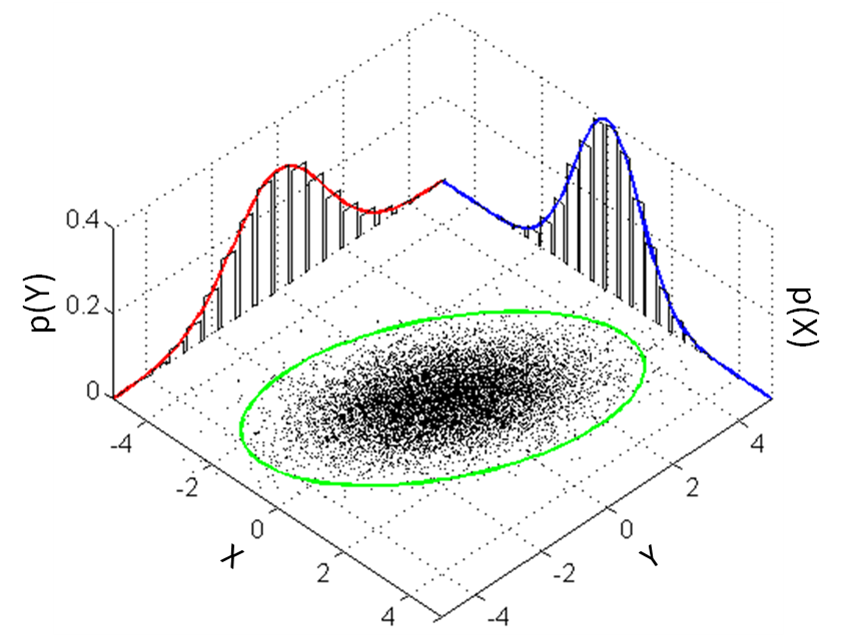
\includegraphics[width=250pt,keepaspectratio]{figures/body/methodology/multivariate_normal.png}
    \caption{Multivariate Gaussian Distribution \cite{multivariate_normal_distribution}}
    \label{figure:multivariate_normal}
\end{figure}

With \(k\) number of varieties, and \(\mu\) as the mean, Multivariate Gaussian Distribution's Probability Distribution Function is displayed below:

\begin{displaymath}
f(x) = \frac{1}{(2\pi)^{\frac{k}{2}}\abs{\Sigma}^{\frac{1}{2}}}e^{-\frac{1}{2}(x-\mu)'\Sigma^{-1}(x-\mu)}
\end{displaymath}

\hfill

In this project, data for Multivariate Gaussian Distribution was generated through NumPy's \path{random.multivariate_normal()} function. The first required input of the mean was given through randomly generating a value within specified parameters (\autoref{section:random_number_generation}). The second required input was a 2-D array represented a co-variance matrix, whose data was generated with the use of Uniform Distributions (\autoref{subsubsection:uniform_distribution}).

\subsection{Use Cases}
Histogram generation utilizes the greatest number of Continuous Probability Distributions. It has an equally random chance of using Gaussian, Lognormal, Gamma, Weibull and Uniform Distributions, all of which can be seen in \autoref{figure:histogram_distributions}.

\hfill

\begin{figure}
    \centering
    \begin{subfigure}[b]{0.19\textwidth}    
        \centering
        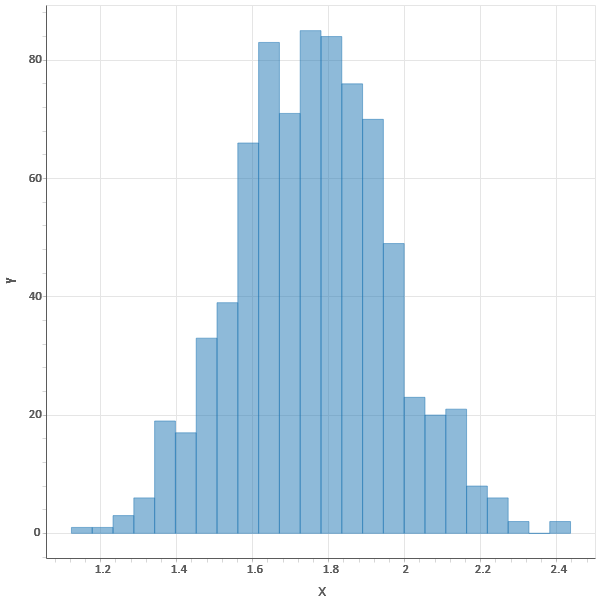
\includegraphics[width=\textwidth]{figures/body/methodology/norm_hist.png}
        \label{figure: norm_hist}
        \caption{Gaussian}
    \end{subfigure}
    \hfill
    \begin{subfigure}[b]{0.19\textwidth}
        \centering
        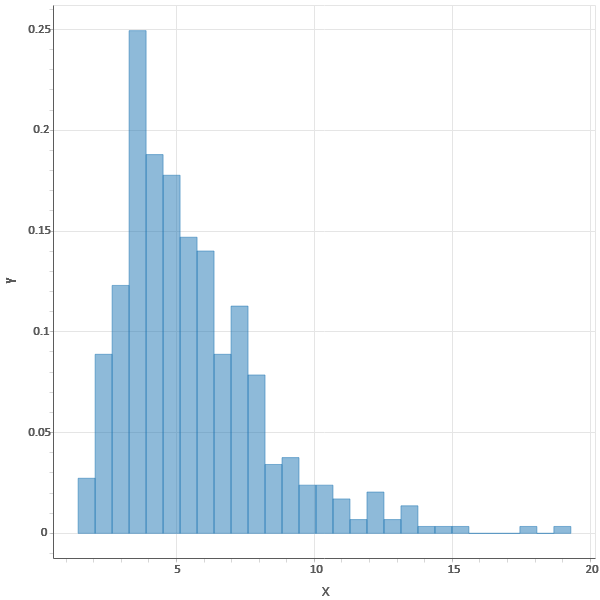
\includegraphics[width=\textwidth]{figures/body/methodology/lognorm_hist.png}
        \label{figure: lognorm_hist}
        \caption{Lognormal}
    \end{subfigure}
    \hfill
    \begin{subfigure}[b]{0.19\textwidth}
        \centering
        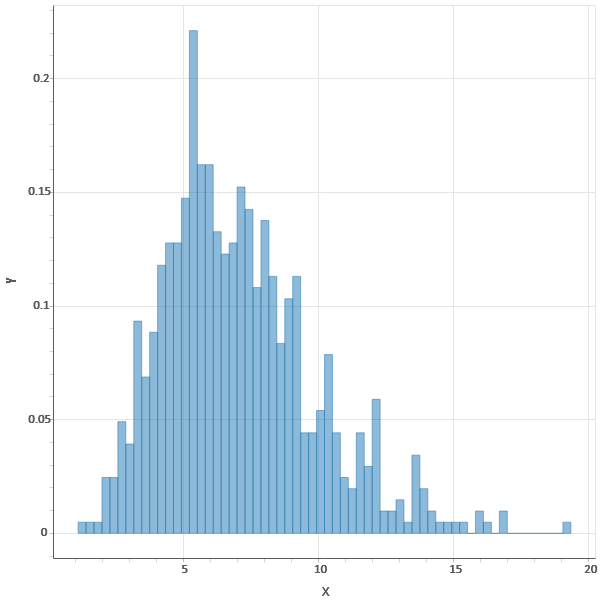
\includegraphics[width=\textwidth]{figures/body/methodology/gamma_hist.png}
        \label{figure: gamma_hist}
        \caption{Gamma}
    \end{subfigure}
    \hfill
    \begin{subfigure}[b]{0.19\textwidth}
        \centering
        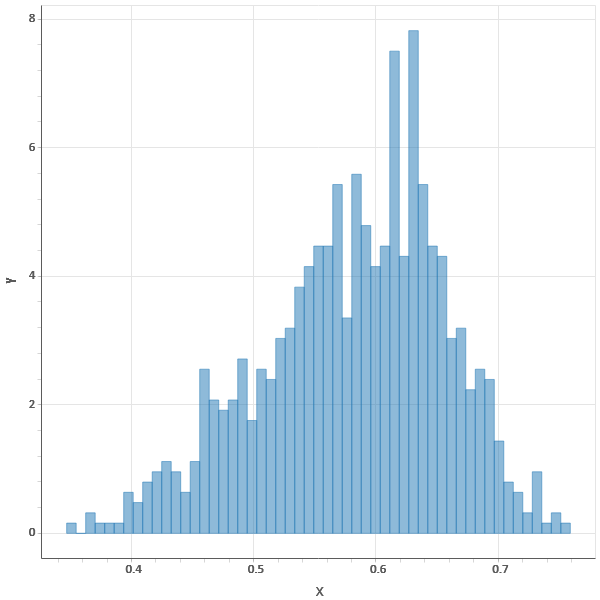
\includegraphics[width=\textwidth]{figures/body/methodology/weibull_hist.png}
        \label{figure: weibull_hist}
        \caption{Weibull}
    \end{subfigure}
    \hfill
    \begin{subfigure}[b]{0.19\textwidth}
        \centering
        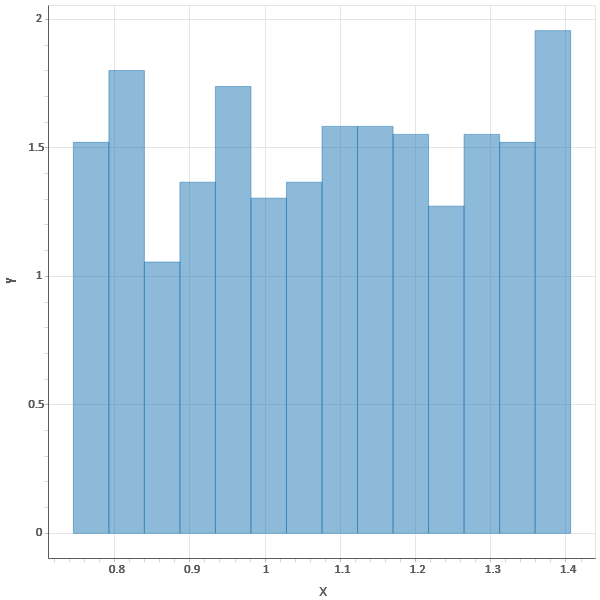
\includegraphics[width=\textwidth]{figures/body/methodology/uniform_hist.png}
        \label{figure: uniform_hist}
        \caption{Uniform}
    \end{subfigure}
    \caption{2-D Continuous Probability Distributions - Histogram}
    \label{figure:histogram_distributions}
\end{figure}

Gaussian Distribution was also applied for kernel density estimation, box and violin plots, which resulted in graphs such as the ones displayed in \autoref{figure:normal_distribution}.

\hfill

\begin{figure}
    \centering
    \begin{subfigure}[b]{0.29\textwidth}
        \centering
        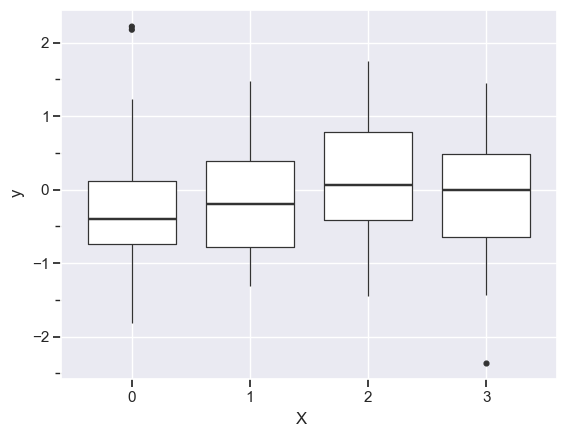
\includegraphics[width=\textwidth]{figures/body/methodology/norm_box.png}
        \caption{Box Plot}
        \label{figure:norm_box}
    \end{subfigure}
    \begin{subfigure}[b]{0.29\textwidth}
        \centering
        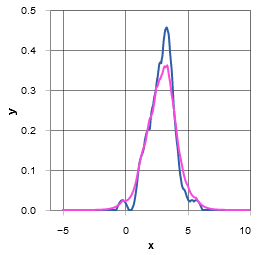
\includegraphics[width=\textwidth]{figures/body/methodology/norm_kde.png}
        \caption{KDE Plot}
        \label{figure:kdeplot}
    \end{subfigure}
    \begin{subfigure}[b]{0.29\textwidth}
        \centering
        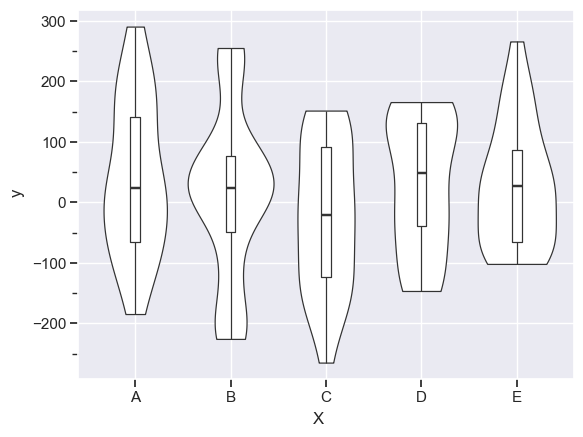
\includegraphics[width=\textwidth]{figures/body/methodology/norm_violin.png}
        \caption{Violin Plot}
        \label{figure:norm_violin}
    \end{subfigure}
    \caption{Gaussian Distributions}
    \label{figure:normal_distribution}
\end{figure}

The only graph type to use Multivariate Gaussian Distribution was contour plot, as it graphs a multi-dimensional surface, demonstrated in \autoref{figure:multivariate_contour}.

\hfill

\begin{figure}[hbt]
    \centering
    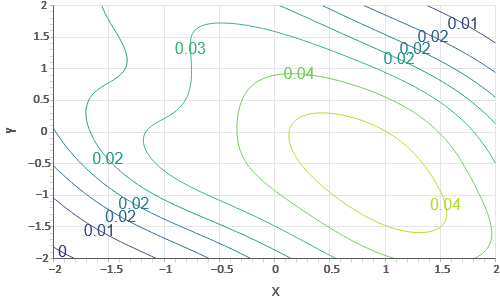
\includegraphics[width=250pt,keepaspectratio]{figures/body/methodology/multi_contour.png}
    \caption{Multivariate Gaussian Distribution - Contour}
    \label{figure:multivariate_contour}
\end{figure}

\section{Geometric Brownian Motion}
Geometric Brownian Motion, also named Exponential Brownian Motion, was not implemented in this project for a variety of reasons. Not only was it difficult to implement and more predictable than other generation methods, but it also would only be used for line graphs. Nevertheless, if this project was to be expanded, then the implementation of methods such as Geometric Brownian Motion should be added. It is due to this logic that Geometric Brownian Motion's generation and possible use case shall continue to be discussed.

\begin{figure}[hbt]
    \centering
    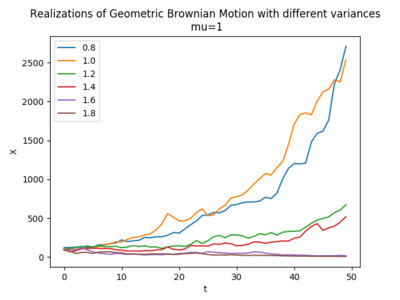
\includegraphics[width=375pt,keepaspectratio]{figures/body/methodology/geometric_example.png}
    \caption{Geometric Brownian Motion - Line Graph \cite{geometric_brownian_motion}}
    \label{figure:geometric_example}
\end{figure}

\subsection{Generation}
Graphs that follow Geometric Brownian Motion typically start at an origin of zero and grow exponentially, with a slight visual appearance of roughness. Since Geometric Brownian Motion is a stochastic process with linear drift, its data follows a stochastic differential equation. This equation is displayed below, where \(W_t\) is the Brownian motion, \(\mu\) is the drift percentage, and \(\sigma\) is the volatility percentage:

\begin{displaymath}
dS_{t} = \mu S_{t}dt + \sigma S_{t}dW_{t}
\end{displaymath}

\hfill

To generate data using this equation, \(W_t\) would be Normally Distributed (\autoref{subsubsection:normal_distribution}), and the rest of the input would be randomly generated within specified ranges (\autoref{section:random_number_generation}).

\subsection{Use Cases}
If Geometric Brownian Motion had been implemented then it would have been used as another correlation type for line graphs. This would have resulted in generations similar to the graph displayed in \autoref{figure:geometric_example}.

\section{Perlin Noise}
Perlin Noise is an extremely powerful pseudo-random generation algorithm used for creating random patterns that appear more ``organic" or lifelike in nature. Moreover, the algorithm is heavily used for procedurally generating content as the generated patterns contain patches, or gradients, of similar values which makes them appear to be only somewhat random. This makes it extremely effective for generating terrain (\autoref{figure:perlin_noise_terrain_mesh}) as well as creating textures for objects such as cloud, marble, or fire, as demonstrated in \autoref{figure:perlin_noise_texture}.

\hfill

\begin{figure}
    \centering
    \begin{subfigure}[b]{0.49\textwidth}
        \centering
        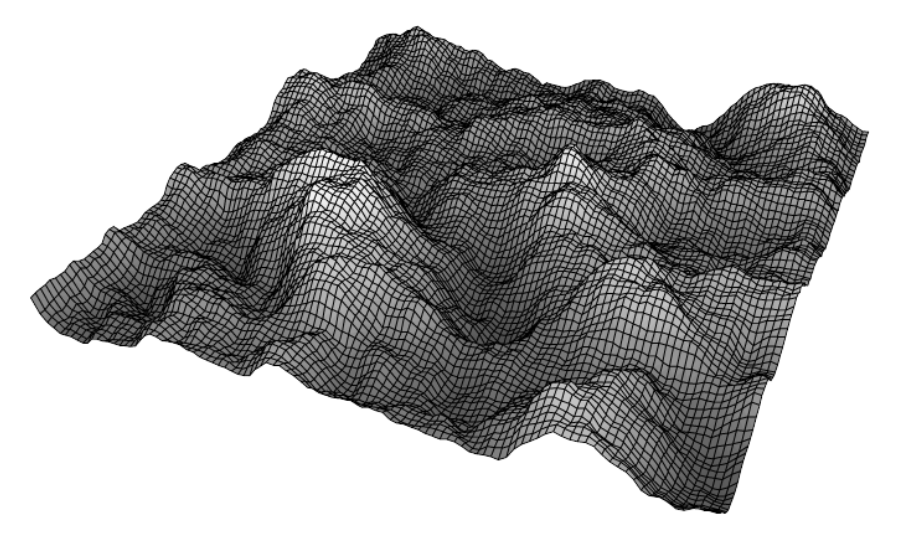
\includegraphics[width=\textwidth]{figures/body/methodology/perlin_noise_terrain_mesh.png}
        \caption{Procedurally Generated Terrain \cite{prunier}}
        \label{figure:perlin_noise_terrain_mesh}
    \end{subfigure}
    \begin{subfigure}[b]{0.49\textwidth}
        \centering
        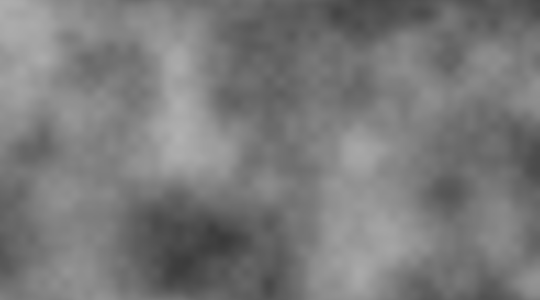
\includegraphics[width=\textwidth]{figures/body/methodology/perlin_noise_texture.png}
        \caption{Perlin Noise Mapped to 2-D Texture \cite{perlin_noise_2007}}
        \label{figure:perlin_noise_texture}
    \end{subfigure}
    \caption{Example Applications of Perlin Noise}
\end{figure}

\subsection{Generation}
While Perlin Noise has a few variations, namely Improved Perlin Noise \cite{perlin_2002} and Simplex noise, the base function remains largely the same. In this particular case, Improved Perlin Noise was further examined and is the topic of discussion below. The summary below is largely influenced by the article authored by Adrian Biagioli \cite{biagioli_2014}.

\hfill

The algorithm begins with a Perlin Noise function. This function takes in an \(x\), \(y\), and \(z\) coordinate as input and outputs a value between 0.0 and 1.0 \cite{gustavson_2005}. To generate this value, the coordinates are first divided into unit cubes to ``normalize" the coordinate within the desired dimension space. A 2-D representation of this can be found in \autoref{figure:perlin_noise_unit_cube}. The 4 corner coordinates of this cube are then utilized to generate a pseudo-random gradient vector. Comparatively, if 3-D Perlin Noise is being generated, this cube would possess 8 unit coordinates rather than the 4 mentioned above. These gradient vectors, as seen in \autoref{figure:perlin_noise_gradient_vector}, will be used to calculate distance vectors from the provided point to the 4 corner points (\autoref{figure:perlin_noise_gradient_distance}).

\hfill

\begin{figure}
    \centering
    \begin{subfigure}[b]{0.29\textwidth}
        \centering
        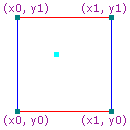
\includegraphics[width=\textwidth]{figures/body/methodology/perlin_noise_unit_cube.png}
        \caption{2-D Unit Cube}
        \label{figure:perlin_noise_unit_cube}
    \end{subfigure}
    \begin{subfigure}[b]{0.29\textwidth}
        \centering
        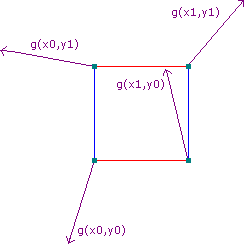
\includegraphics[width=\textwidth]{figures/body/methodology/perlin_noise_gradient_vector.png}
        \caption{Gradient Vectors}
        \label{figure:perlin_noise_gradient_vector}
    \end{subfigure}
    \begin{subfigure}[b]{0.29\textwidth}
        \centering
        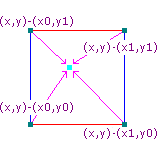
\includegraphics[width=\textwidth]{figures/body/methodology/perlin_noise_gradient_distance.png}
        \caption{Distance Vectors}
        \label{figure:perlin_noise_gradient_distance}
    \end{subfigure}
    \caption{Generation Steps of Perlin Noise \cite{biagioli_2014}}
    \label{figure:perlin_noise_generation}
\end{figure}

Next, the dot product between each gradient vector and it's corresponding distance vector are computed, creating an influence value. This value is positive when it is in the direction of the gradient, negative when opposite facing, and has a value of 0 if both vectors are perpendicular (\autoref{figure:perlin_noise_influence}). All influence values in the grid must then be interpolated to create a value much like a weighted average. One final step, known as easing, must be completed due to the linear interpolation, as the averaged values would otherwise look unnatural. 

\hfill

\begin{figure}
    \centering
    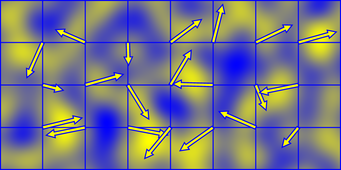
\includegraphics[width=0.6\textwidth]{figures/body/methodology/perlin_noise_influence.png}
    \caption{2-D Representation of Perlin Noise Influence Values \cite{biagioli_2014}}
    \label{figure:perlin_noise_influence}
\end{figure}

A fade function, or ease curve, is used on the averaged coordinate values to create a smoother transition between gradients \autoref{figure:perlin_noise_ease}. By using this ease curve, the coordinates are changed more gradually when approaching integral coordinates, thus creating patterns that seem to flow together. The easing function used in the Improved Perlin Noise algorithm can be seen below, where \(t\) represents a given unit cube coordinate.

\begin{displaymath}
6t^5 - 15t^4 + 10t^3
\end{displaymath}

\begin{figure}
    \centering
    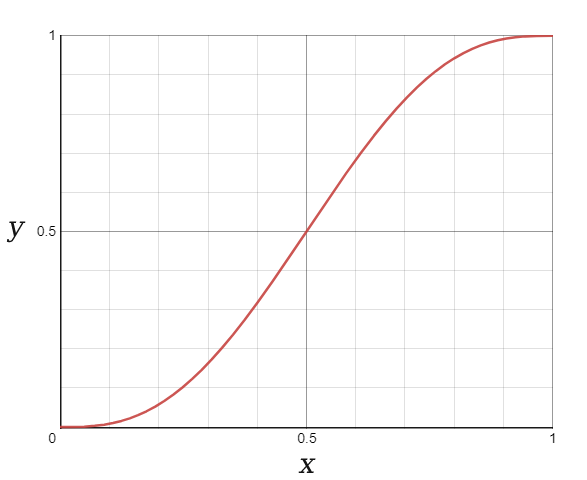
\includegraphics[width=0.55\textwidth]{figures/body/methodology/perlin_noise_ease.png}
    \caption{Improved Perlin Noise easing function}
    \label{figure:perlin_noise_ease}
\end{figure}

\subsection{Use Cases}
In the context of graph generation, Perlin Noise could be used for generating area graphs as well as contour plots. The former was attempted to be implemented, however, in testing, the data did not provide examples visually similar to a standard contour plot. However, it is still believed that Perlin Noise could be used to generate random contour plots, as the following articles by Benjamin Hauer \cite{hauer_2019} and Amit Patel \cite{patel_2015} seemingly do so, although further research must be conducted before reaching any final conclusions. As it is commonly used in terrain generation, for both 2-D and 3-D environments, it is no surprise that Perlin Noise is feasible for generating adequate area plots. Due to the aforementioned roadblocks, as well as stringent time constraints, Perlin Noise was not further researched for either contour or area graph generation. 

\hfill

Additional implementations such as CONREC \cite{bourke_1987}, a subroutine for contouring a specified surface as a triangular mesh, and Simplex noise \cite{gustavson_2005}, an enhanced version of the original Perlin Noise algorithm, were also considered and subsequently discarded. The aforementioned CONREC algorithm was extremely hard to randomize and did not provide representative contour plots which is ultimately why it was rejected.

\hfill

On the other hand, the Simplex noise algorithm does alleviate some of the problems with Perlin Noise, such as computational complexity and an inequal direction distribution, however, it was abandoned for the same reasons faced by Perlin Noise. While it is believed that CONREC and simplex noise could still be used for contour generation, similar to Perlin Noise, further research must be completed before reaching a conclusion.

\section{Random Number Generation}
\label{section:random_number_generation}
Random Number Generation allows for integers and floats to be randomly generated. This is useful for data generation, stylization, theming, and randomizing input parameters.

\subsection{Generation}
Random Number Generation produces a random value, or a range of data points with seemingly no pattern or correlation in a specified range. Depending on the type of variable desired, either NumPy's \path{random.randint()} or NumPy's \path{random.uniform()} method was applied for generation, which utilizes Uniform Distributions (\autoref{subsubsection:uniform_distribution}) to return random values. Since its input parameters require a smallest possible integer and a largest possible integer, these parameters were also randomly generated within a previously specified range.

\subsection{Use Cases}
As Random Number Generation was heavily relied upon during this project, there were a large variety of factors and use cases it was responsible for. The first of which was simply to generate data with no correlation, which was utilized in line graphs, error bar graphs and bar charts. This data generation can be seen in \autoref{figure:rand_num_data_gen}.

\hfill

\begin{figure}
    \centering
    \begin{subfigure}[b]{0.32\textwidth}
        \centering
        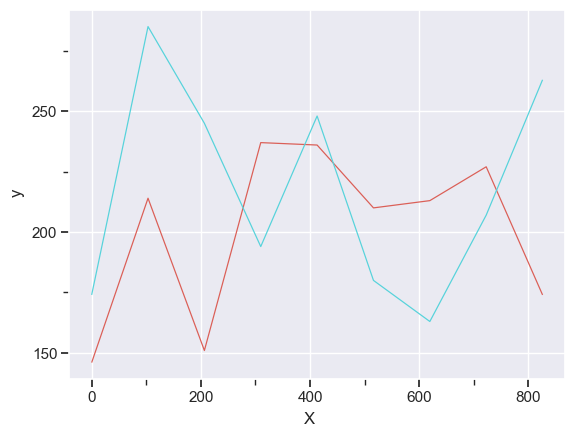
\includegraphics[width=\textwidth]{figures/body/methodology/random_line.png}
        \caption{Line Graph}
        \label{figure:random_line}
    \end{subfigure}
    \hfill
    \begin{subfigure}[b]{0.32\textwidth}
        \centering
        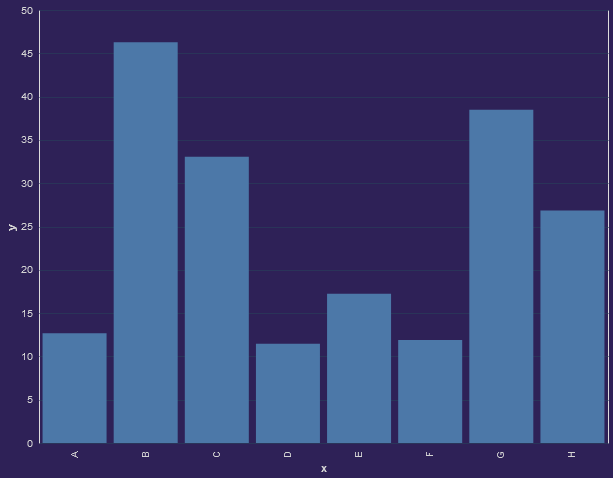
\includegraphics[width=\textwidth]{figures/body/methodology/random_bar.png}
        \caption{Bar Chart}
        \label{figure:random_bar}
    \end{subfigure}
    \hfill
    \begin{subfigure}[b]{0.32\textwidth}
        \centering
        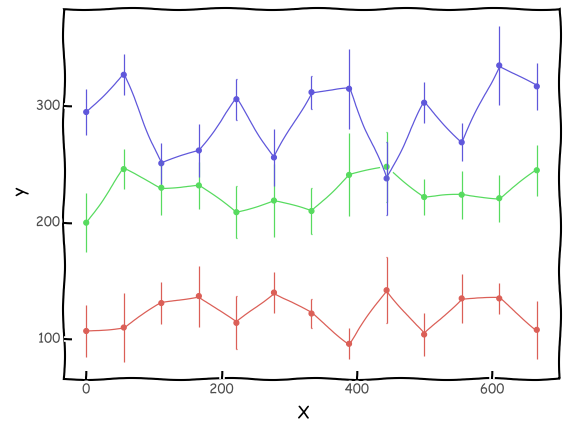
\includegraphics[width=\textwidth]{figures/body/methodology/random_error.png}
        \caption{Error Bar}
        \label{figure:random_error}
    \end{subfigure}
    \caption{Random Number Graph Generation}
    \label{figure:rand_num_data_gen}
\end{figure}

It is also worth noting that correlation for bar charts were generated by ordering the random data points. This resulted in the addition of positive and negative correlations, each with a random amount of noise and a random chance of displaying horizontally rather than vertically. These correlations are displayed in \autoref{figure:bar_correlations}.

\hfill

\begin{figure}
    \centering
    \begin{subfigure}[b]{0.24\textwidth}
        \centering
        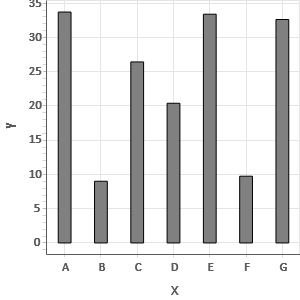
\includegraphics[width=\textwidth]{figures/body/methodology/random_vertical_bar.png}
        \caption{Random Vertical}
        \label{figure:random_vertical_bar}
    \end{subfigure}
    \hfill
    \begin{subfigure}[b]{0.24\textwidth}
        \centering
        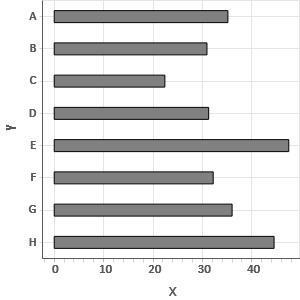
\includegraphics[width=\textwidth]{figures/body/methodology/random_horizontal_bar.png}
        \caption{Random Horizontal}
        \label{figure:random_horizontal_bar}
    \end{subfigure}
    \hfill
    \begin{subfigure}[b]{0.24\textwidth}
        \centering
        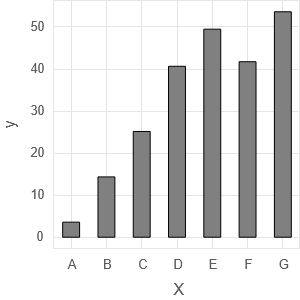
\includegraphics[width=\textwidth]{figures/body/methodology/pos_vertical_bar.png}
        \caption{Positive Vertical}
        \label{figure:pos_bar}
    \end{subfigure}
    \hfill
    \begin{subfigure}[b]{0.24\textwidth}
        \centering
        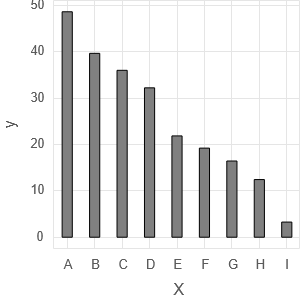
\includegraphics[width=\textwidth]{figures/body/methodology/neg_vertical_bar.png}
        \caption{Negative Vertical}
        \label{figure:neg_error}
    \end{subfigure}
    \caption{Bar Chart Random Correlations}
    \label{figure:bar_correlations}
\end{figure}

In addition to data points, Random Number Generation was used to generate graph-specific input, such as graph orientation and number of layers, lines, boxes, or violins. Another example of this is graphs that required specific sizes per data point, such as bubble size or error bar length. Furthermore, any random input parameters needed for generation functions were created using Random Number Generation, with the ranges predetermined by the user.

\hfill

Lastly, Random Number Generation was used for theming and stylization purposes in order to further graph type variation. Themes were randomly picked per library, and examples of random stylization include line thickness, colour (RGB values ranging between 0 and 255), as well as marker sizes. More information on theming and stylization can be found in \autoref{subsection:style_generation}.